% !TeX root = 00main.tex

%%%%%%%%%%%%%%%%%%%%%%%%%%%%%%%%%%%%%%%%%%%%%%%%%%
% System design
%%%%%%%%%%%%%%%%%%%%%%%%%%%%%%%%%%%%%%%%%%%%%%%%%%

In this section, we discuss the overall layout of the system, the electronic and mechanical design and the software.

%%%%%%%%%%
% Overall design  
%%%%%%%%%%

\subsection*{Overall design}

The design is based on the initial proposal by Matsubara-san, with some modifications to ease installation and improve the coverage of the light on the PMT~array. The cables, electronics, and housing were manufactured by Interface2~Ltd.\cite{INTERFACE2}.

\subsubsection*{System configuration}
%
% System configuration
%

Figure~\ref{figure:controlbox} shows the overall layout of the system. The LEDs are mounted on next to the PMTs, on the boards holding them. The system consists of six `branches': a cable string with a data and power line that at certain intervals holds a `pulserhead': an electronics board with digital logic and an ultra-fast LED pulser. Each string has either two or three pulserheads. In total, there are twelve pulserheads with a 420~nm LED and two pulserheads with a 355~nm LED (the 355~nm light will be absorbed almost immediately and emitted randomly in all directions as a longer wavelength). Each branch is terminated with a connector containing a 120~$\Omega$ resistor on the data line. 

The cable exit the experiment through four flanges. The cables, made out of (expensive) teflon coated cables are then connected to a junction box, where they connected to (cheap) 15~m long ethernet cables. These cables are connected to the nanopulser control box, located in the DAQ racks. The controller box talks to the DAQ via the network (ssh to the raspberry pi inside the controller box). The junction box is grounded and a ground cable connects to the controller box as well. The controller box also provides a trigger signal in-sync with the optical pulse. There are programmable delays that control the timing between the optical pulse and the trigger pulse for each of the pulserheads. 

\begin{figure}
\begin{center}	
  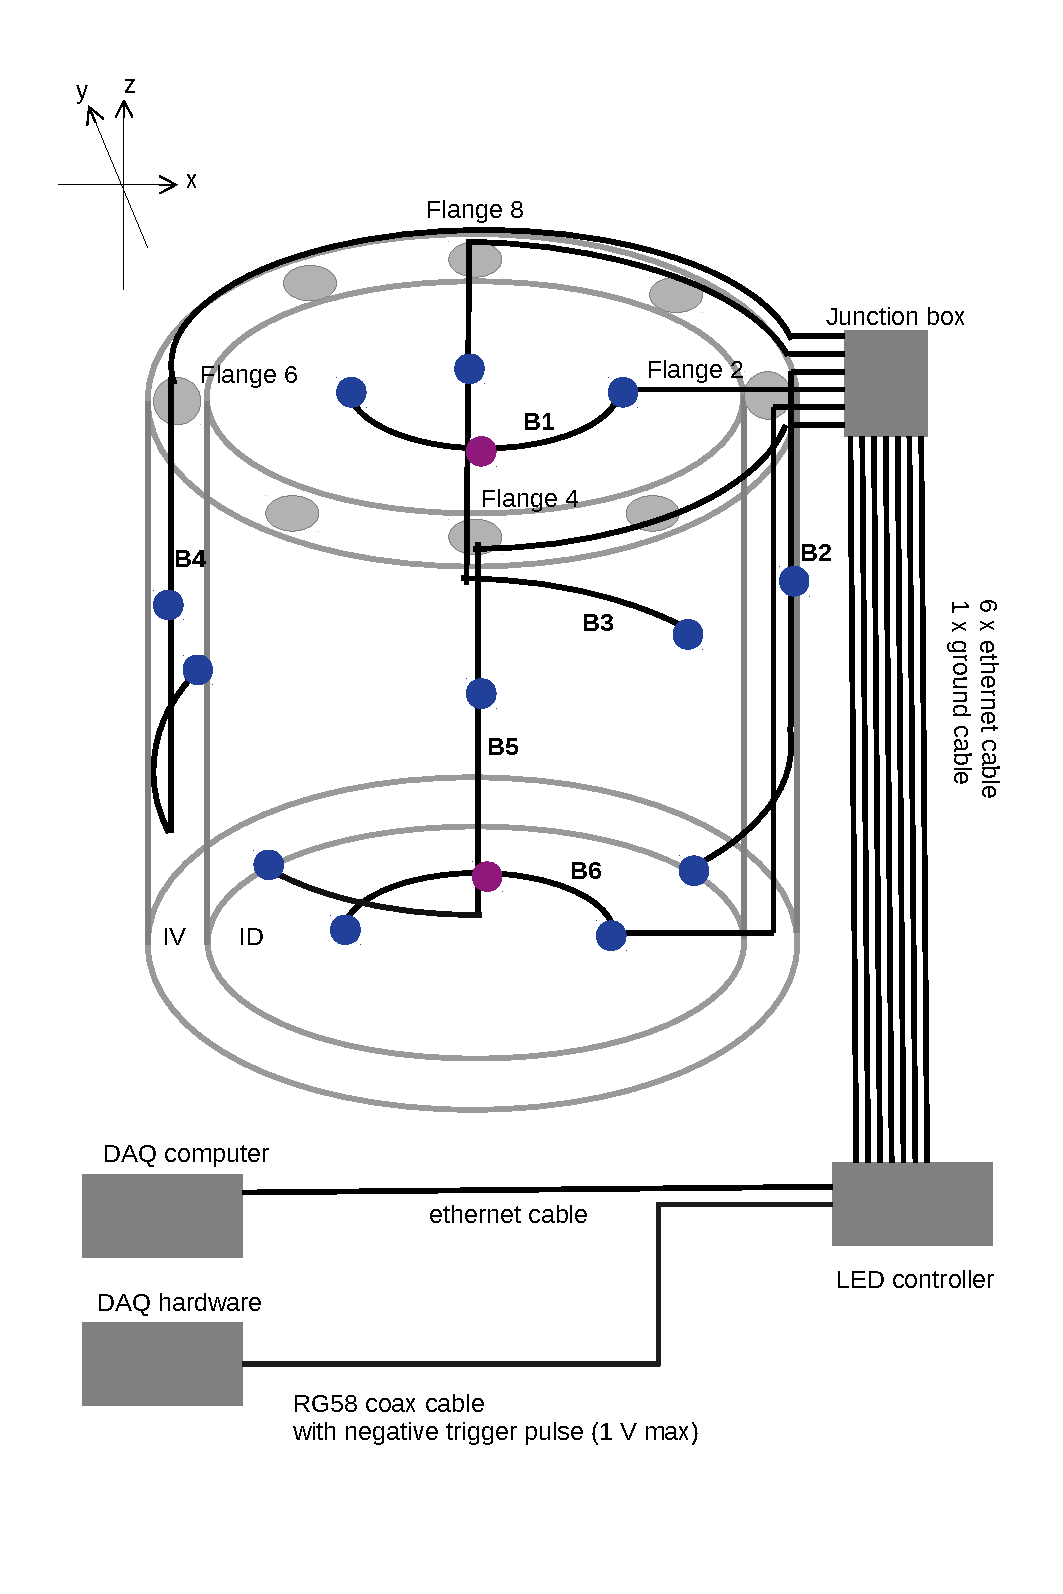
\includegraphics[width=0.75\linewidth]{figures/JSNS2_led_system_overview.pdf}
  \caption{A schematic overview of the nanopulser optical calibration system. The (two) purple points indicate the position of the pulserheads (LED driver boards) with a 355~nm LED, the (twelve) blue points indicate pulserheads with a 420~nm LED. All LEDs point inwards. The numbers B1-B6 indicated the different branches. IV is the Inner Veto volume and ID is the Inner Detector volume.}
  \label{figure:controlbox}
\end{center}
\end{figure}

Table~\ref{table:cable_configuration} shows the overall configuration of the branches, as well as the branch and the pulserhead IDs. Furuta-san has produced a paper indicating the exact mounting pounts.

\fix[inline]{SJMP: add docdb entry for Furuta-san's document, once on docdb}

\begin{table}[h!]
  \begin{center}
    \caption{Configuration of the \jsns nanopulser optical calibration system, up to the junction box.}
    \label{table:cable_configuration}
    \begin{tabular}{|c|c|c|c|c|c|c|c|c|c|c|c} 
	\hline
	 &  & Cable  & \multicolumn{2}{c|}{Pulserhead} &  Cable & \multicolumn{2}{c|}{Pulserhead} &  Cable & \multicolumn{2}{c|}{Pulserhead}\\ \cline{4-5} \cline{7-8} \cline{10-11}
	Branch & Flange & length (m) &  ID & $\lambda_{\mathrm{LED}}$ (nm) & length (m) &  ID & $\lambda_{\mathrm{LED}}$ (nm) & length (m) &  ID & $\lambda_{\mathrm{LED}}$ (nm) \\ \hline
	1 & 2 & 5.5   &  1 & 420 & 2.2 & 2 & 355 & 2.2 & 3 & 420 \\ 
	2 & 2 & 4.5   &  4 & 420 & 3.0 & 5 & 420 & & & \\ 
	3 & 2 & 9.0   &  6 & 420 & 3.0 & 7 & 420 & & & \\ 
	4 & 2 & 13.5 &  8 & 420 & 3.0 & 9 & 420 & & & \\ 
	5 & 2 & 9.0   & 10 & 420 & 3.0 & 11 & 420 & & & \\ 
	6 & 2 & 10    & 12 & 420 & 2.2 & 13 & 355 & 2.2 & 14 & 420 \\
	\hline
    \end{tabular}
  \end{center}
\end{table}

\begin{figure}
\begin{center}	
  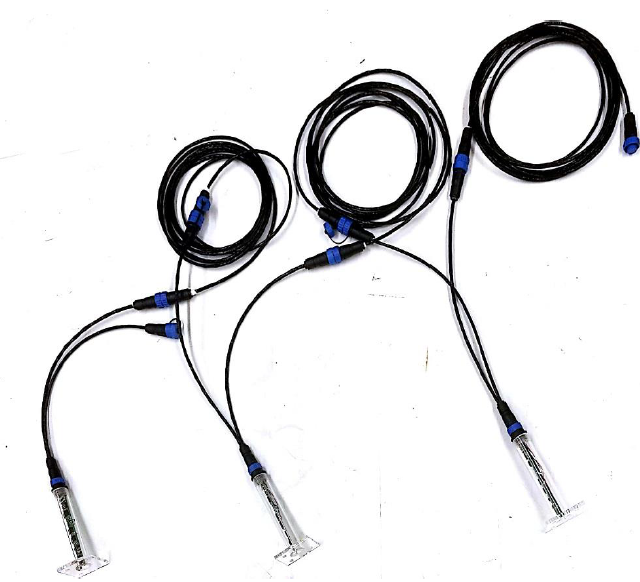
\includegraphics[width=0.5\linewidth]{figures/branch.png}
  \caption{A picture of one of the \jsns nanopulser branches.}
  \label{figure:branch}
\end{center}
\end{figure}

The cables for the branches are teflon-coated with four twisted-pairs wires inside, and a grounding shield. The connectors are Bulgin buccanneer 400~\cite{BULGIN}. The O-rings used are TRP White FFKM~\cite{TRP} (all the orignal connector O-rings were been replaced with FFKM O-rings). 

All materials used in the branches (up to the junction box) have been shown to be compatible with LAB (see monthly meeting reports). 
It has also been shown that the branches can be safely deployed into liquid, for up to 2~bar over pressure (at least).


%
% System configuration
%

\subsubsection*{System performance}

%%%%%%%%%%
% Nanopulser head
%%%%%%%%%%

\subsection*{Pulserhead}

\begin{figure}
\begin{center}	
  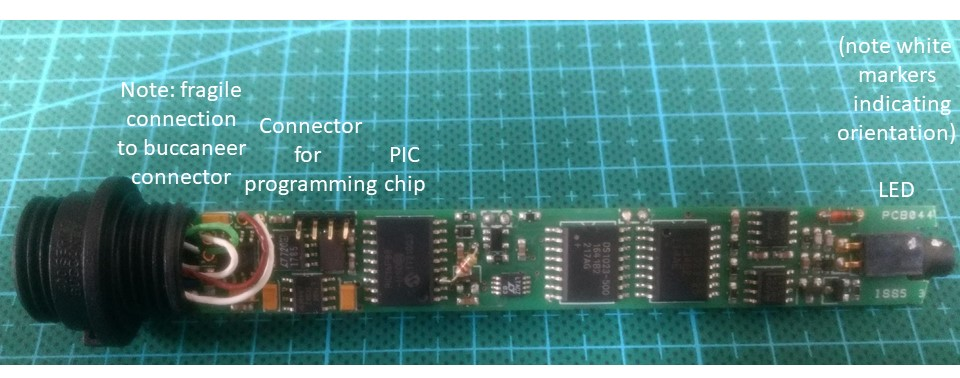
\includegraphics[width=1.0\linewidth]{figures/pulserhead.jpg}
  \caption{Photo of the a pulserhead, outside of its acrylic housing, with the main components indicated.}
  \label{figure:pulserhead}
  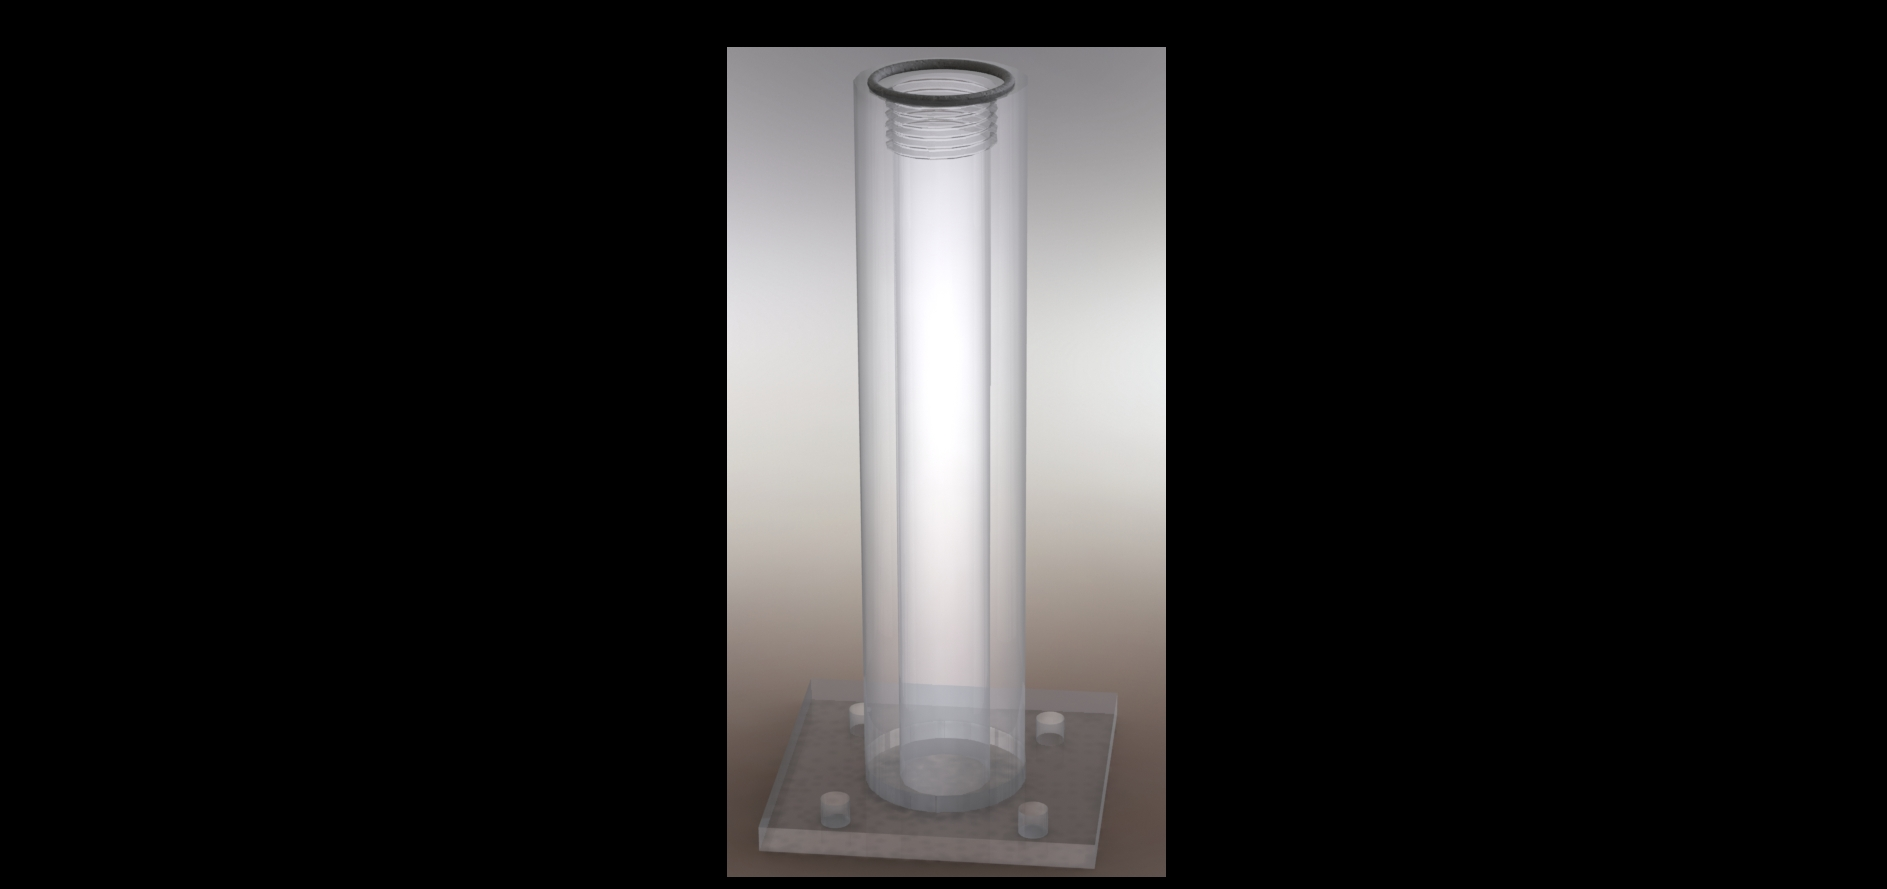
\includegraphics[width=0.75\linewidth]{figures/PulserTube2.jpg}
  \caption{Rendered drawing of the acrylic housing, with an O-ring (black in this image, but white in reality).}
  \label{figure:pulserhead_housing}
\end{center}
\end{figure}

Note that for transfer the maximum energy in a fast pulse, that we found that it is important that the legs of the LEDs are not shortened, but bend out to fit.

A detailed schematic is given in Appendix~\ref{app:schematics}. The glue used is in the assembly is Weldon~42~\cite{WELDON}.

The LED emission (in air) was close to a Lambertian distribution~\cite{LAMBERTIAN}. This corresponds an opening angle of LEDs of approximately 30~degrees. However, this depends on the selection of light, and on the individual LEDs. 

\begin{figure}
\begin{center}	
  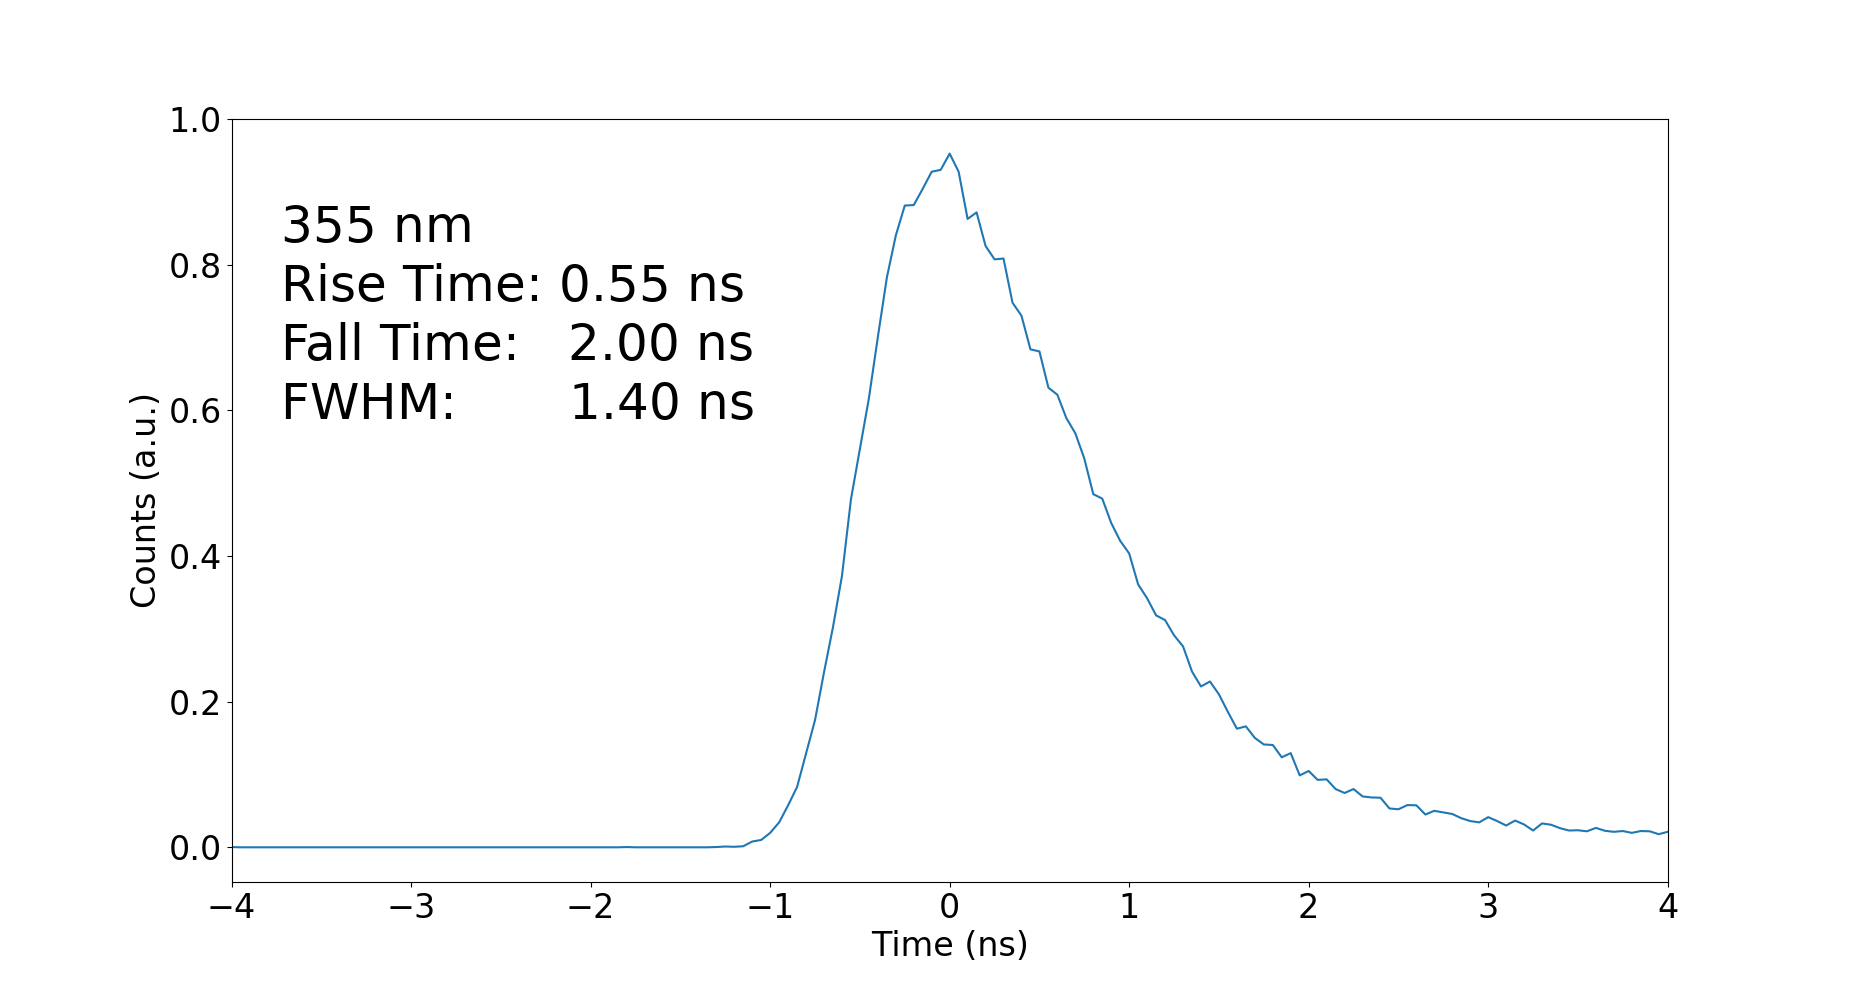
\includegraphics[width=0.60\linewidth]{figures/355_nm_2.png}
  \caption{The nominal optical pulse shape of the 355~nm pulserhead.}
  \label{figure:355nmperf}
  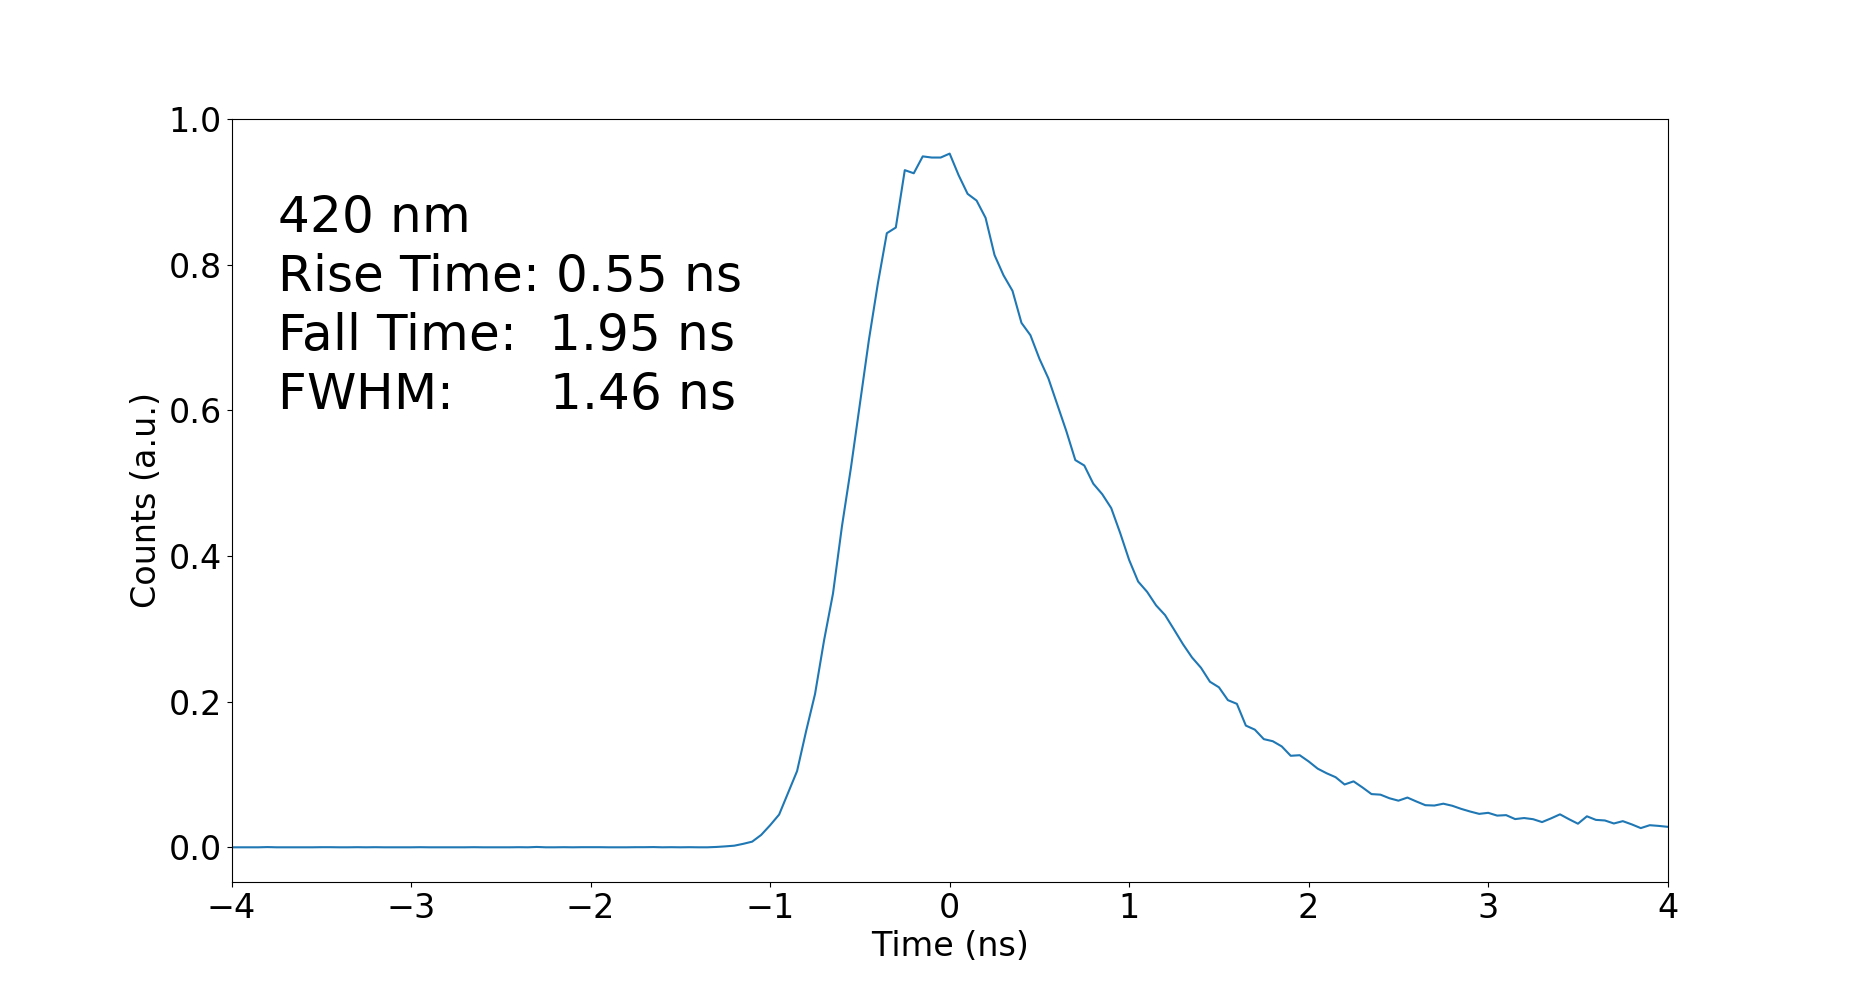
\includegraphics[width=0.60\linewidth]{figures/420_nm_2.png}
  \caption{The nominal optical pulse shape of the 420~nm pulserhead.}
  \label{figure:420nmperf}
\end{center}
\end{figure}

The wavelength distribution of the LEDs is reasonably well described by a `double Gaussian', with a mean of either 355~nm or 420~nm, and a lower sigma of 10~nm and a higher sigma of 15~nm. The exact spectra is given in Figures~\ref{figure:355nmspec}~and~\ref{figure:420nmspec}. (The input data for these figures is provided in \label{app:led_spectra} for reference.)

%
% Data in:
% C:\Users\sjp39\OneDrive - University of Sussex\20 RESEARCH\JSNS2\LED system\Design documents
% 5mmLED_SprectralPlots.xlsx, analysed with plot_spectra.ipynb
%

\begin{figure}
\begin{center}	
  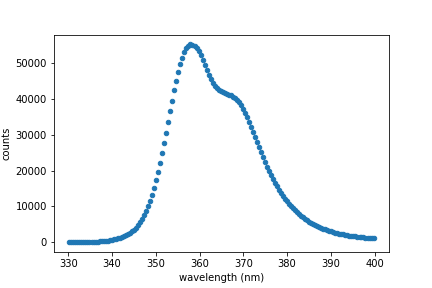
\includegraphics[width=0.60\linewidth]{figures/led_uv.png}
  \caption{The optical spectrum of the 355~nm pulserhead.}
  \label{figure:355nmspec}
  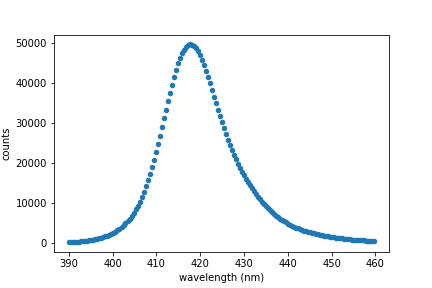
\includegraphics[width=0.60\linewidth]{figures/led_blue.png}
  \caption{The optical spectrum of the 420~nm pulserhead.}
  \label{figure:420nmspec}
\end{center}
\end{figure}

%
% Nanopulser head programming
%
\subsubsection*{Pulserhead programming}

The Pulserheads are each programmed for a specific position on the branch and with its own unique ID (1-14). The programming can be done separately from the system, as shown in Figure~\ref{figure:pulserhead_programming}, with a custom cable providing the 9~V power for the PIC chip\footnote{Make sure the battery has enough power left to power the PIC chip.}. The code is loaded onto the PIC~chip via a commercial interface (microchip PICkit3) with a custom cable to the pulserhead. Note that, as shown in Figure~\ref{figure:pulserhead_programming}, the grey lead lines up with the arrow on the PICkit3 interface. On the other side, the green lead is closest to the LED on the pulserhead. The connector on the pulserhead is slanted an slightly bend, to make it fit into the pulserhead's acrylic housing. Therefore, take extra care when connecting to make sure a good contact is make.

The software for the pulserhead programming can be found on github~\cite{GITHUB_PIC}. This contains a zip file (PICkit3.zip), which contains the windows compatible executable file PICkit3.exe, as well as other (required) input files for the program. It also contains the 14 hex files to be loaded onto the pulser: nanoSlaveTrig\_X.hex, where X is a letter from A-N. This corresponds to pulser ID 1-14, respectively, as shown in Table%~\ref{table:cabling_overview}
 (i.e., A is for pulser head 1, etc.).

The program PICkit3.exe is started by double-clicking (make sure the PICkit3 device is connected and recognised, otherwise the next step is not possible). Next, select the PIC chip to program: under menu `Device family', select {\bf MidRange}. Then, under `Device', select {\bf PIC16F88} (note there are a lot of models). If the set-up is correct, you can now read the PIC chip by pressing the 'Read' button. This take a little and a green progress bar will appear until the commend read has finished. This should change the hex values shown in Program Memory from their default values to all different values. 

If this was successful, load a hex file by clicking `Import Hex' from the `File' menu. Next, click `Write'. Again a green progress bar should appear to show the progress. Wait until the process has been completed. After this, the PIC chip has been programmed and can be disconnected from the power supply and the PICkit3 device.

\begin{figure}
\begin{center}	
  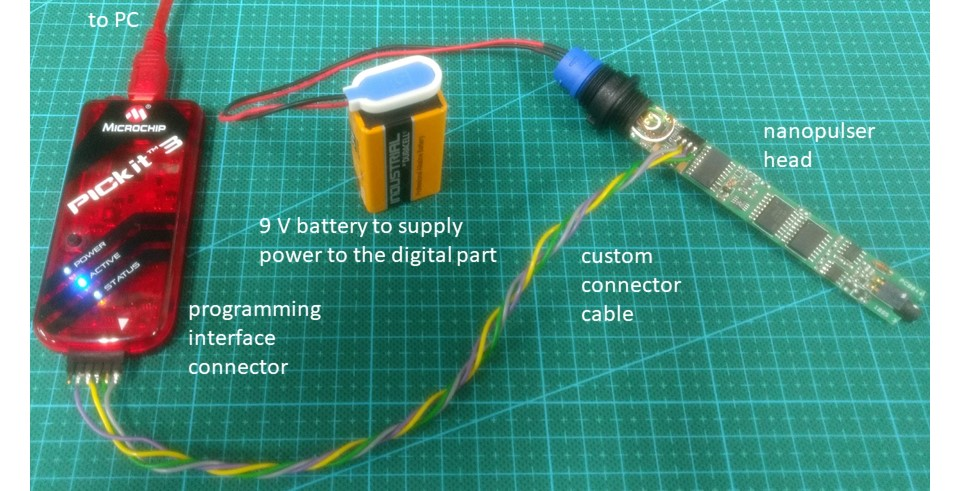
\includegraphics[width=1.0\linewidth]{figures/pulserhead_programming.jpg}
  \caption{The pulserhead programming set-up (window10 computer needed, not shown here).}
  \label{figure:pulserhead_programming}
\end{center}
\end{figure}

The perfomance of the pulserheads is documented on github\cite{GITHUB_TEST}, and is summarised in Figure~\ref{figure:pulserhead_output}.

\begin{figure}
\begin{center}	
  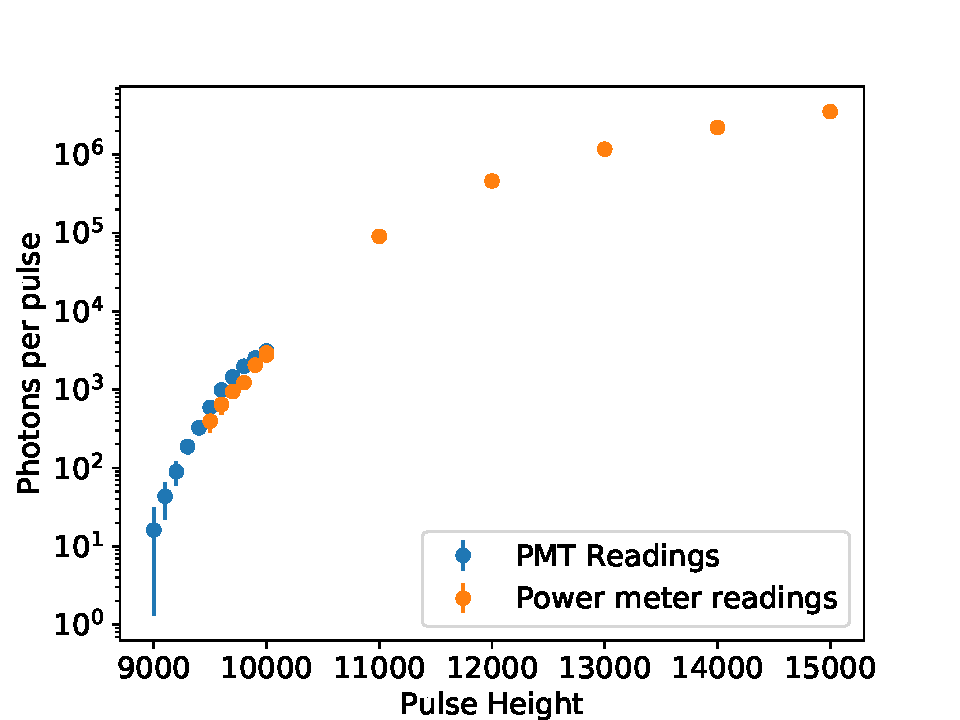
\includegraphics[width=0.48\linewidth]{figures/PhotonCounts420nm.pdf}
  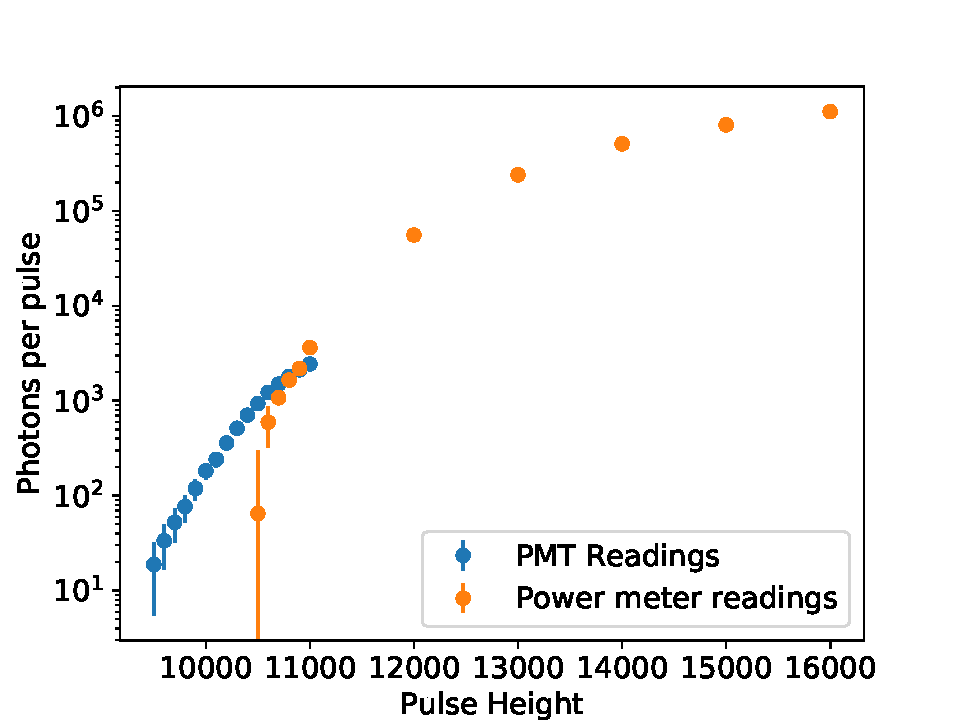
\includegraphics[width=0.48\linewidth]{figures/PhotonCounts355nm.pdf}
  \caption{The optical output of the pulserheads with 420~nm LEDs (left) and 355~nm LEDs (right). The x-axis is the digital setting used for the measurements. Most of the range is observed with a calibrated optical power meter. At the low end, however, this device was not sensitive enough and a careful extrapolation based on measurement using a PMT is shown.}
  \label{figure:pulserhead_output}
\end{center}
\end{figure}

%%%%%%%%%%
% Nanopulser control box
%%%%%%%%%%

\subsection*{Nanopulser control box}

\begin{figure}
\begin{center}	
  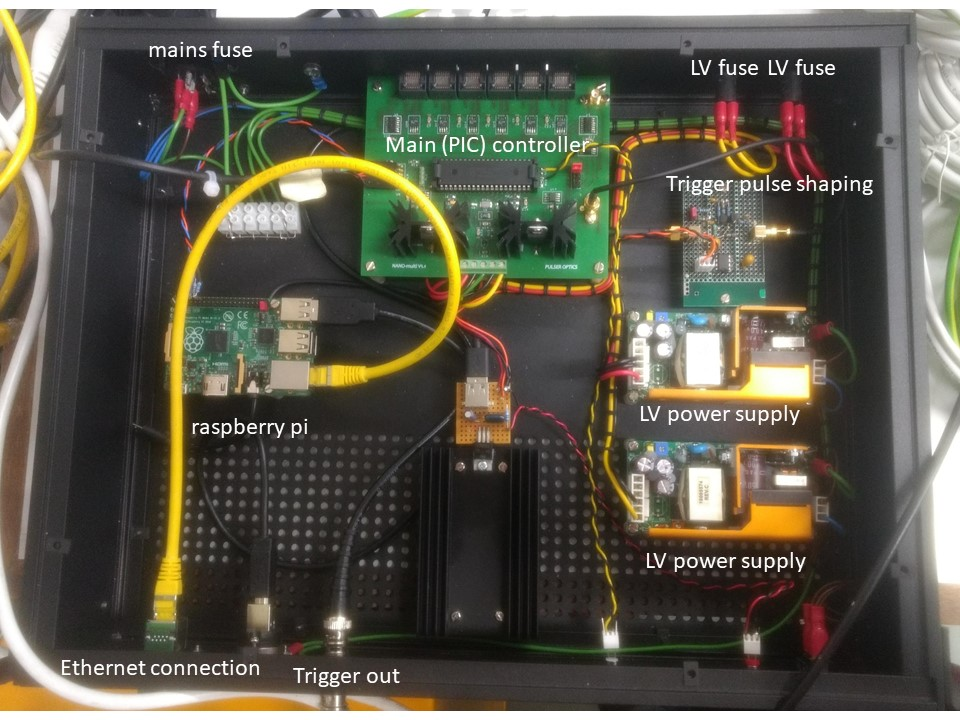
\includegraphics[width=0.75\linewidth]{figures/controlbox.jpg}
  \caption{Photo of the control box during commissioning at the University of Sussex, with the main components indicated. Note that all the fuses and connections can be accessed from the outside.}
  \label{figure:controlbox}
\end{center}
\end{figure}

One symptom of a blown fuse can be that  the pulser does communicate but either does not produce light, or produces a wide pulse (of the order of 100~ns).

The control box has two indicator lights: a red light and a green light.
The red light is connected to the 5~V supply to indicate the unit is powered up. 
The green light is labeled ‘active’, and indicates that any one of the slave units is emitting light.


\subsection*{Cable design}

The ethernet cables should {\bf never} be unplugged from the box, while the power is on, as the power for both the digital electronics, as well as for the pulser circuits runs through them. Note: accidental hot-swapping can result in one of the fuses blowing. Therefore, always power the system off before connecting or disconnecting the ethernet cables to the control box.

\subsection*{Junction box}

\begin{figure}
\begin{center}	
  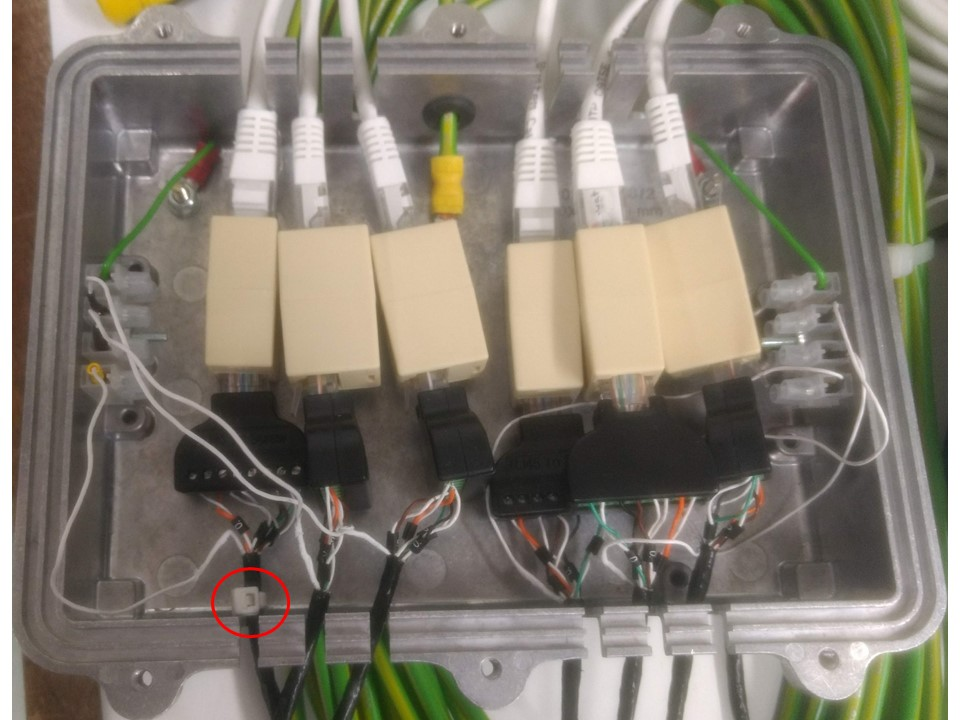
\includegraphics[width=0.75\linewidth]{figures/junction_box.jpg}
  \caption{Photo of the junction during commissioning at the University of Sussex. The ethernet cables on the top connect to the back of the control box (this is labeled 1-6 for the branch numbers). The cables coming from the connector need to be wired to the black eight-way connectors in the pictures (details given below). The cables are then connected with the beige mating connectors. After final assembly in the flange, a tie wrap should be wrapped on each cable as a strain relief. This is demonstrated in the bottom left cable (red circle). }
  \label{figure:junction_box}
\end{center}
\end{figure}

\begin{figure}
\begin{center}	
  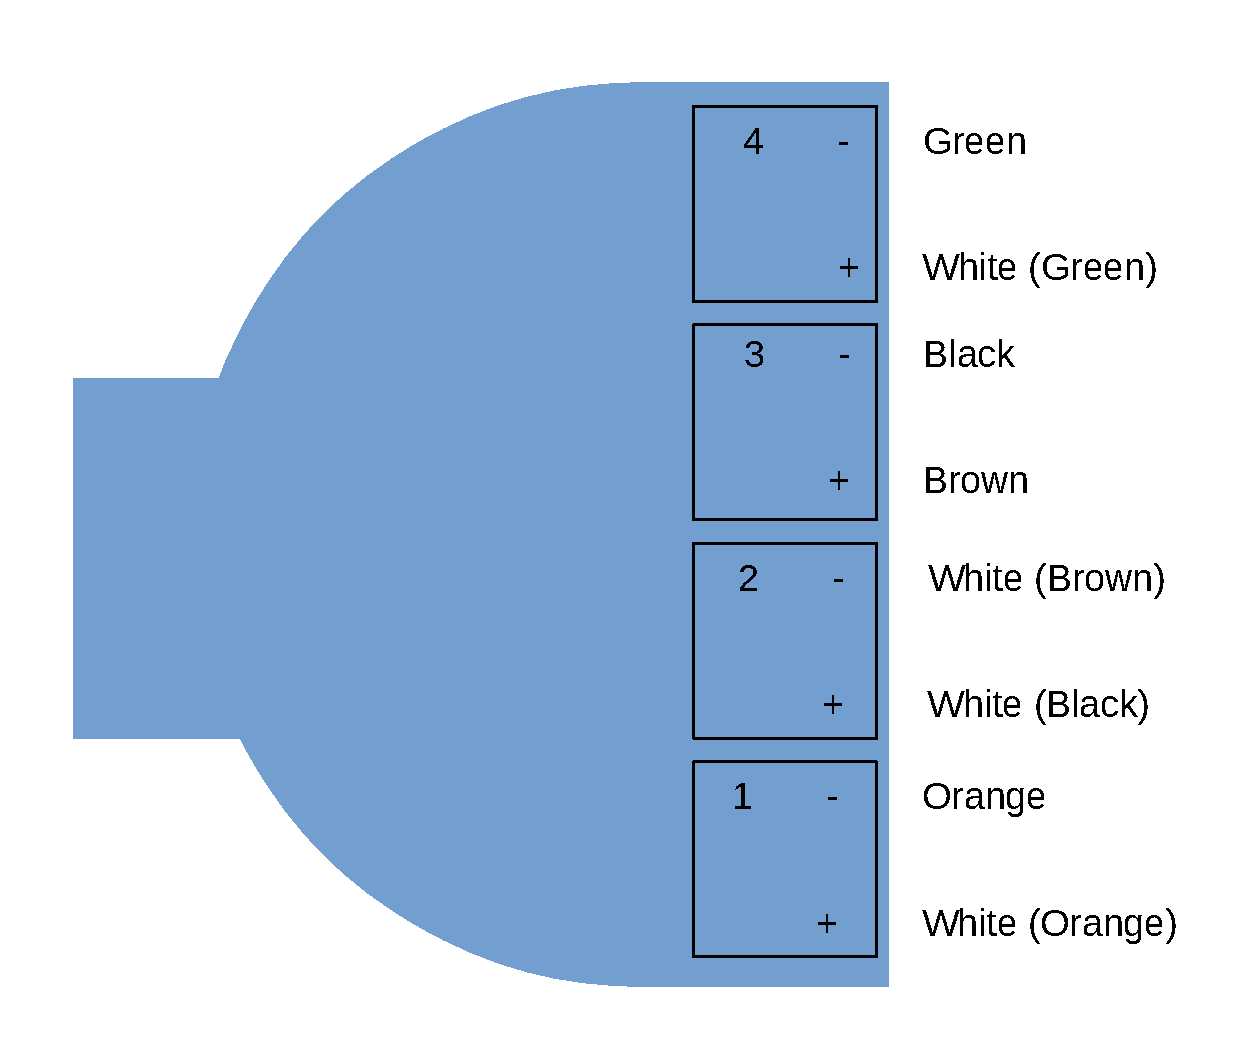
\includegraphics[width=0.5\linewidth]{figures/connector.pdf}
  \caption{A diagram indication how the eight-way connector should be connected to the cables going into the vessel.}
  \label{figure:connector}
\end{center}
\end{figure}

At the final installation, the cables should be wrapped with a tie wrap inside the junction box, to avoid damage to the connection by accidentally pull the cables. Note that the (longer) ground cable also needs to be connected to the junction box chassis (see Figure~\ref{figure:junction_box}).

\subsection*{Trigger delay}
When the slave board receives a `run' command, it outputs a (trigger) pulse, which is sent back to the control board. The time it takes to receive by the control board depends on the cable length. This pulse is internally delayed on the slave board before triggering the LED driver circuit. The delay is preset using two delay lines of step size 5~ns (called `course trigger delay') and 0.25~ns (called `fine trigger delay'). By matching the total delay to the cable length, the trigger pulse received at the control box (or beyond) can be made co-incident with the light pulse. The number of programmable steps is 255 for each delay line. Thus the maximum delay is 1,338.75~ns (1275~ns plus 63.75~ns).

%%%%%%%%%%
% Nanopulser control  software
%%%%%%%%%%

\subsection*{Control software}

The software is kept in a  github repository\cite{GITHUB_SOFT}.
(An older, depricated, version with documentation is also kept in a different github repository\cite{GITHUB_TEST}, for reference only).
 
A raspberry pi computer, which runs the control software, is situated within the control box. To operate the box you need to ssh into the raspberry pi using \texttt{ssh pi@<IP address>}. The MAC address of the raspberry pi ethernet port is \texttt{b8:27:eb:ef:45:ee}.

The control software for the driver board are located in the folder: \texttt{/home/pi/JSNS2PulserControl/ControlSoftware/}.
The script to control the driver boards is: \texttt{\textbf{test\_run.py}}.
It takes the following arguments:\\
\newline
\texttt{\textbf{-c}} - The pulserhead ID to pulse \newline
\texttt{\textbf{-p}} - The pulse height for the driver board, this controls the intensity of each LED pulse. (Ranges from 0 to 16384)\newline
\texttt{\textbf{-d}} - The delay between pulses in milliseconds \newline
\texttt{\textbf{-n}} - Number of pulses. The number of pulses must be a multiple of 1000, up to 65,025
\newline
All arguments are required for this example scripts. (Note that continuous running is not possible for this system, but it is in the library. Also, the coarse and fine fibre delays are set to default values in this script.) The python scripts making up the control software provide detailed information on the possible commands.
